%%%%%%%%%%%%%%%%%%%%%%%%%%%%%%%%%%%%%%%%%
% University Assignment Title Page 
% LaTeX Template
% Version 1.0 (27/12/12)
%
% This template has been downloaded from:
% http://www.LaTeXTemplates.com
%
% Original author:
% WikiBooks (http://en.wikibooks.org/wiki/LaTeX/Title_Creation)
%
% License:
% CC BY-NC-SA 3.0 (http://creativecommons.org/licenses/by-nc-sa/3.0/)
% 
% Instructions for using this template:
% This title page is capable of being compiled as is. This is not useful for 
% including it in another document. To do this, you have two options: 
%
% 1) Copy/paste everything between \begin{document} and \end{document} 
% starting at \begin{titlepage} and paste this into another LaTeX file where you 
% want your title page.
% OR
% 2) Remove everything outside the \begin{titlepage} and \end{titlepage} and 
% move this file to the same directory as the LaTeX file you wish to add it to. 
% Then add \input{./title_page_1.tex} to your LaTeX file where you want your
% title page.
%
%%%%%%%%%%%%%%%%%%%%%%%%%%%%%%%%%%%%%%%%%

%----------------------------------------------------------------------------------------
%	PACKAGES AND OTHER DOCUMENT CONFIGURATIONS
%----------------------------------------------------------------------------------------

\documentclass[12pt]{article}

\usepackage[utf8]{inputenc}
\usepackage[T1]{fontenc}
\usepackage{lmodern}
\usepackage{parselines}
\usepackage[portuguese]{babel}
\usepackage{graphicx}
\usepackage[document]{ragged2e}
\usepackage{listings}
\usepackage{xcolor}
\usepackage[margin=0.8in]{geometry}		
\usepackage{amsmath}
\usepackage{hyperref}
\usepackage{url}
\usepackage{float}
\usepackage{titlesec}
\usepackage{hyperref}
\usepackage{booktabs}
\usepackage{pgfplots}
\usepackage{animate}
\usepackage{listings}
\usepackage{color}

\definecolor{dkgreen}{rgb}{0,0.6,0}
\definecolor{gray}{rgb}{0.5,0.5,0.5}
\definecolor{mauve}{rgb}{0.58,0,0.82}

\lstset{frame=tb,
  language=Java,
  aboveskip=3mm,
  belowskip=3mm,
  showstringspaces=false,
  columns=flexible,
  basicstyle={\small\ttfamily},
  numbers=none,
  numberstyle=\tiny\color{gray},
  keywordstyle=\color{blue},
  commentstyle=\color{dkgreen},
  stringstyle=\color{mauve},
  breaklines=true,
  breakatwhitespace=true,
  tabsize=3
}

\pgfplotsset{compat=1.5}
\graphicspath{ {images/} }

\titleclass{\subsubsubsection}{straight}[\subsection]

\newcounter{subsubsubsection}[subsubsection]
\renewcommand\thesubsubsubsection{\thesubsubsection.\arabic{subsubsubsection}}
\renewcommand\theparagraph{\thesubsubsubsection.\arabic{paragraph}} % optional; useful if paragraphs are to be numbered

\titleformat{\subsubsubsection}
  {\normalfont\normalsize\bfseries}{\thesubsubsubsection}{1em}{}
\titlespacing*{\subsubsubsection}
{0pt}{3.25ex plus 1ex minus .2ex}{1.5ex plus .2ex}

\makeatletter
\renewcommand\paragraph{\@startsection{paragraph}{5}{\z@}%
  {3.25ex \@plus1ex \@minus.2ex}%
  {-1em}%
  {\normalfont\normalsize\bfseries}}
\renewcommand\subparagraph{\@startsection{subparagraph}{6}{\parindent}%
  {3.25ex \@plus1ex \@minus .2ex}%
  {-1em}%
  {\normalfont\normalsize\bfseries}}
\def\toclevel@subsubsubsection{4}
\def\toclevel@paragraph{5}
\def\toclevel@paragraph{6}
\def\l@subsubsubsection{\@dottedtocline{4}{7em}{4em}}
\def\l@paragraph{\@dottedtocline{5}{10em}{5em}}
\def\l@subparagraph{\@dottedtocline{6}{14em}{6em}}
\makeatother

\setcounter{secnumdepth}{4}
\setcounter{tocdepth}{4}

\begin{document}

\begin{titlepage}

\newcommand{\HRule}{\rule{\linewidth}{1mm}} % Defines a new command for the horizontal lines, change thickness here

\center % Center everything on the page
 
%----------------------------------------------------------------------------------------
%	HEADING SECTIONS
%----------------------------------------------------------------------------------------


\includegraphics{feup.jpg}

\textsc{\large Agentes e Inteligência Artificial Distribuída}\\[0.8cm] % Major heading such as course name
\textsc{\large 4º ano do Mestrado Integrado em Engenharia Informática e Computação}\\[0.8cm] % Minor heading such as course title

%----------------------------------------------------------------------------------------
%	TITLE SECTION
%----------------------------------------------------------------------------------------

\HRule \\[1.2cm]
{ \huge \bfseries Simulação dinâmica da gestão de AGVs num contexto fabril}\\[0.6cm] % Title of your document
\HRule \\[3cm]
 
%----------------------------------------------------------------------------------------
%	AUTHOR SECTION
%----------------------------------------------------------------------------------------


% If you don't want a supervisor, uncomment the two lines below and remove the section above
\Large \emph{Authors:}\\[0.5cm] \normalsize
Daniel \textsc{Reis}\\[0.1cm] - up201308586 
- up201308586@fe.up.pt\\[0.1cm]
David \textsc{Baião}\\[0.1cm] - up201305195
- up201305195@fe.up.pt\\[0.1cm] 
Filipa \textsc{Ramos}\\[0.1cm] - up201305378
- up201305378@fe.up.pt\\[3cm] % Your name

%----------------------------------------------------------------------------------------
%	DATE SECTION
%----------------------------------------------------------------------------------------

{\large \today}\\[0cm] % Date, change the \today to a set date if you want to be precise

%----------------------------------------------------------------------------------------
%	TABLE OF CONTENTS & LISTS OF FIGURES AND TABLES
%----------------------------------------------------------------------------------------

\tableofcontents

%----------------------------------------------------------------------------------------
%	INTRODUÇÃO
%----------------------------------------------------------------------------------------

\section{Introdução} 

\justify\normalsize
No âmbito da unidade curricular de Agentes e Inteligência Artificial Distribuída pretende-se simular as operações de uma fábrica que utiliza AGVs para transporte de peças entre máquinas nas variadas fases de produção. Serão utilizadas plataformas de sistema e/ou frameworks na construção e simulação de agentes. O objectivo é manusear estas ferramentas por forma a auxiliar a construção de um sistema multiagente que permite comunicação e negociação entre agentes. Tem-se em vista a exploração das possibilidades destas plataformas atraves da construção de agentes com funções diferentes que se complementam uns aos outros e formam uma unidade de produção fabril.

Este projecto tem como objectivo principal a demonstração de possíveis aplicações de agentes de inteligência artificial no mundo prático. Unidades de produção como a que este projecto envisiona poderão ser uma realidade num futuro proximo e permitirão uma subida exponencial na eficiência e na organização de fabricas de produção em massa.

%----------------------------------------------------------------------------------------

\newpage % Start the article content on the second page, remove this if you have a longer abstract that goes onto the second page

%----------------------------------------------------------------------------------------
%	ESPECIFICAÇÃO
%----------------------------------------------------------------------------------------

\section{Especificação}

\subsection{Descrição do cenário}
Numa fábrica, existem variadas máquinas responsáveis pelas várias etapas da produção. Um lote é composto por um número variável de peças correspondendo, por exemplo, numa fábrica textil, a 10 camisolas. Um lote está pronto quando todas as suas peças passaram por todas as fases da linha de produção. A linha de produção é constituída por máquinas pertencentes a cada uma das fases específicas. Cada fase tem uma ou mais máquinas que fazem o mesmo trabalho. Sempre que uma máquina acaba de processar um lote negoceia com as máquinas responsáveis pela etapa seguinte a transferência do lote em causa. Após a determinação da máquina destino para a próxima etapa, a máquina de origem requere o transporte do lote a um AGV. Após ser feita uma negociação com todos os AGV's presentes no espaço, o escolhido transporta o lote para a máquina destino.

\begin{figure}[H]
  \centering
    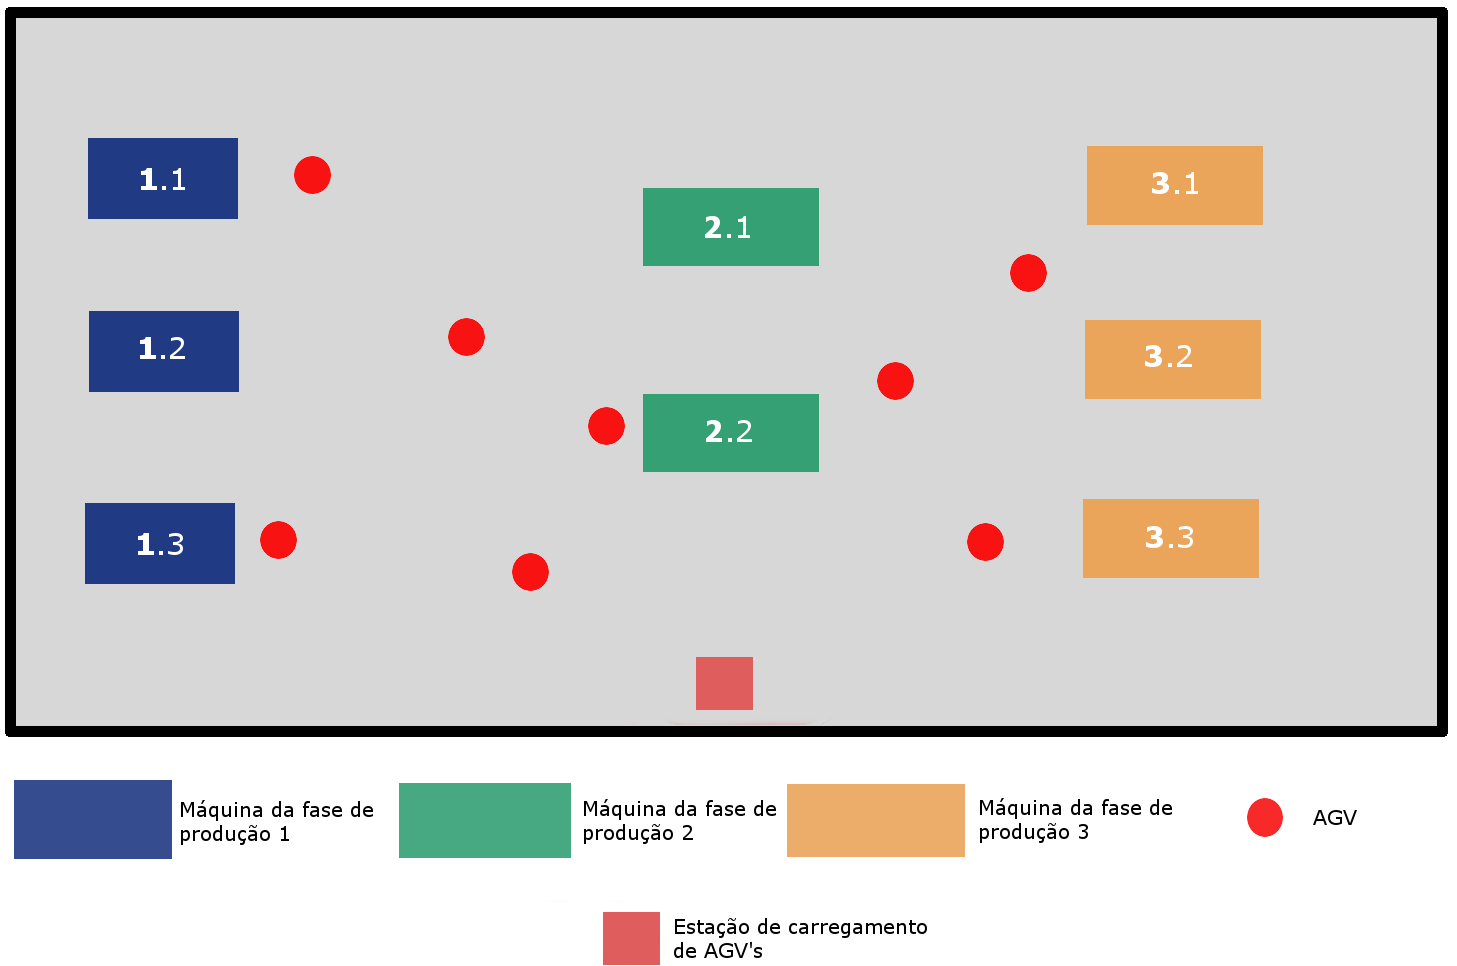
\includegraphics[width=18cm, height = 10.5cm]{scenario.png}
  \caption{Cenário exemplificativo de uma fábrica simples.}
  \label{scenario}
\end{figure}

Como se pode observar no exemplo da figura \ref{scenario}, o processo de fabrico de um lote implica 3 fases distintas. Um lote entraria numa das máquinas da fase 1 e, quando o processo nesta fosse completado, a máquina que processou o lote negoceia com as máquinas da fase 2 para jogar com a disponibilidade das mesmas. Este processo repete-se até o lote ter sido processado numa máquina da última etapa. 

\newpage
Este cenário é constituído por:

\begin{description}
\item[Fase 1] 3 máquinas
\item[Fase 2] 2 máquinas 
\item[Fase 3] 3 máquinas
\end{description}

A negociação entre máquinas é feita na passagem da fase 1 para a fase 2 e da fase 2 para a fase 3. Os círculos vermelhos simbolizam AGV's em diferentes posições do espaço físico da fábrica. A negociação pelo transporte de um AGV implica a análise por parte do agente da distância do AGV à máquina origem e destino. O quadrado presente na parte inferior do esquema representa a estação de carregamento de um AGV. Este não é um agente. É apenas a localização referência para onde os AGV's se deslocam por forma a voltarem a encher a sua bateria.

Para efeitos de transporte por parte de um AGV será considerado que todas as peças de todos os lotes têm o mesmo peso (todos os lotes são compostos por peças iguais).

O espaço físico da unidade fabril está mapeada em coordenadas (\textit{xy}) que auxiliam à localização de todos os elementos do sistema.

\subsubsection{Máquinas}

No início, cada lote tem uma máquina da fase 1 aleatoriamente assignada de acordo com a capacidade de cada máquina. Para o caso da fábrica do exemplo da figura \ref{scenario}, as decisões a serem tomadas por cada máquina estão representadas na figura \ref{decisionMach}.\newline\newline

\begin{figure}[H]
  \raggedleft 
    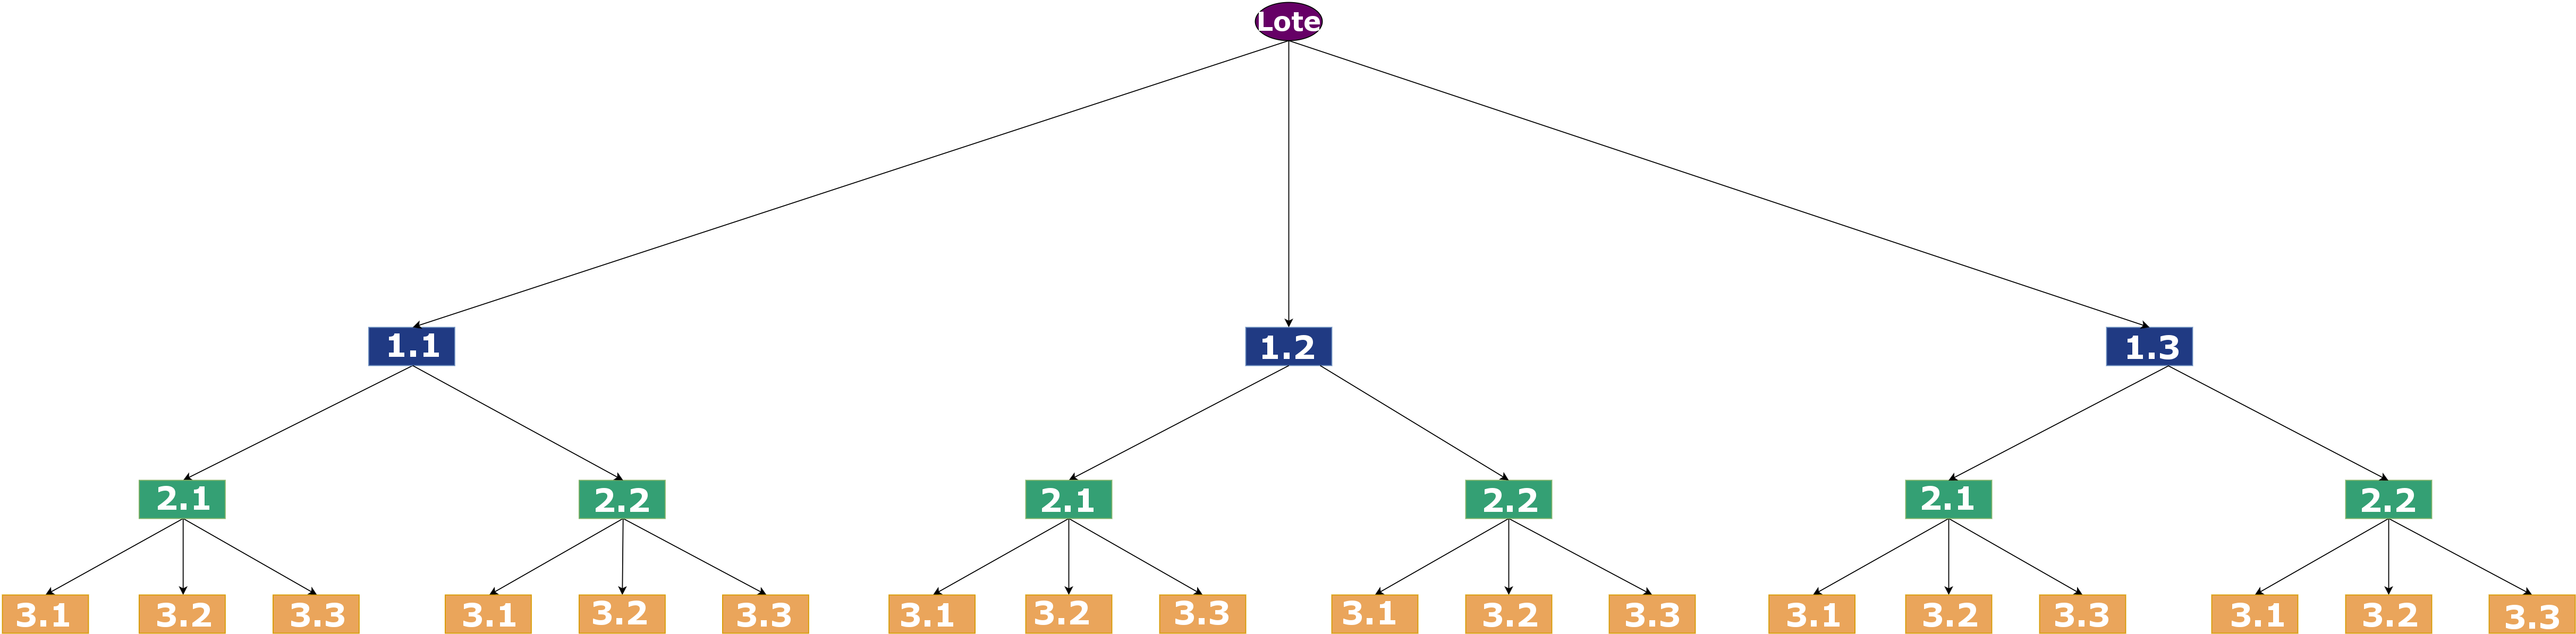
\includegraphics[width=19cm, height = 6cm]{DecisionTreeMachines.png}
  \caption{Árvore de decisão para um lote a ser processado no exemplo \ref{scenario}.}
  \label{decisionMach}
\end{figure}

No processo de decisão sao tidas em conta as variáveis de cada máquina. Cada máquina é caracterizada por:

\begin{description}
\item[Capacidade de processamento] -  Número inteiro de lotes que a máquina consegue processar ao mesmo tempo;
\item[Velocidade de processamento] - Inteiro que avalia a velocidade com que a máquina processa um lote;
\item[Manutenção] - Booleano que indica se a máquina está operacional ou em manutenção;
\item[Localização] - Coordenadas da localização fixa da máquina.
\end{description}

Cada máquina pode continuar a receber lotes até que atinja a sua capacidade máxima de processamento. Todas estas variáveis são inerentes a uma máquina. Podem existir máquinas da mesma fase que não tenham as características iguais. A velocidade é a variável que auxilia ao cálculo do menor tempo em que os lotes são processados. Ao ser feita a escolha da máquina destino são tidos em conta tanto a capacidade de processamento como a velocidade de cada máquina por forma a obter a combinação que minimiza o tempo total de produção do lote.

\subsubsubsection{Grau de Potencial}

O \textbf{Grau de Potencial} de uma máquina expressa o equilíbrio entre as variáveis \textbf{capacidade de processamento} e \textbf{velocidade de processamento} e caracteriza-se pela fórmula seguinte:

\begin{equation}
G_{p}=\frac{1}{C_{p}}\times t_{p}
\label{eqG}
\end{equation}

em que $t_{p}$ representa: 

\begin{equation}
t_{p}=\frac{1}{V_{p}}
\label{eqT}
\end{equation}

\begin{table}[H]
\centering
\caption{Variáveis presentes nas equações \ref{eqG} e \ref{eqT}.}
\label{my-label}
\begin{tabular}{@{}p{2cm}ll@{}}
\toprule
\multicolumn{1}{c}{\textbf{Variável}} & \textbf{Definição}   & \multicolumn{1}{c}{\textbf{Unidades}} \\ \midrule
\multicolumn{1}{c}{$G_{p}$} & Grau de potencial &  \multicolumn{1}{c}{-}  \\ \midrule
\multicolumn{1}{c}{$C_{p}$} & Capacidade de processamento &  \multicolumn{1}{c}{-}  \\ \midrule
\multicolumn{1}{c}{$t_{p}$} & Tempo de processamento      & \multicolumn{1}{c}{$s$} \\ \midrule
\multicolumn{1}{c}{$V_{p}$} & Velocidade de processamento  & \multicolumn{1}{c}{$lotes/s$} \\ \bottomrule
\end{tabular}
\end{table}

Quanto menor o grau de potencial melhor é a opção. Assim, uma máquina escolhe sempre a máquina da fase seguinte com menor grau de potencial. Um menor grau de potencial significa menor tempo de processamento de um lote e este é o objectivo da unidade fabril. Desta forma, o grau de potencial é inversamente proporcional à capacidade de processamento (observável em baixo) e diretamente proporcional ao tempo de processamento (declive da reta é igual a $C_{p}^{-1}$, observável em baixo).

\begin{tikzpicture}
\centering
  \begin{axis}[ 
    title=Variação do grau de potencial em relação à capacidade de processamento,
    xlabel=$C_{p}$,
    ylabel={$G_{p}$},
  ] 
    \addplot[draw=blue][domain=0:5]{1/x};
  \end{axis}\end{tikzpicture}

\begin{tikzpicture}
\centering
  \begin{axis}[ 
    title=Variação do grau de potencial em relação ao tempo de processamento,
    xlabel=$t_{p}$,
    ylabel={$G_{p}$},
  ] 
    \addplot[draw=blue][domain=0:5]{x};
  \end{axis}\end{tikzpicture}
  
  O grau de potencial impede que uma máquina com maior capacidade e velocidade seja sobrecarregada com lotes para processar enquanto que as outras permanecem desocupadas.

\subsubsection{AGV}

Os AGV's (\textit{Automated Guided Vehicles}) vão estar espalhados pelo espaço físico da fábrica, navegando pelo sistema para os sítios onde são necessários. Efetuam negociações diretas com as máquinas que requerem transporte. Todos os AGV's conhecem as localizações de todas as máquinas desde o início da simulação.\newline

A estação de carregamento de AGV é uma posição física no espaço fabril onde os drones vão para recarregarem a sua bateria. Após um tempo de carregamento no qual o drone está parado na estação, a sua autonomia volta ao valor máximo. Enquanto este se encontra na estação, está indisponível para fazer entregas. Um AGV apenas pode ir à estação recarregar quando não puder fazer qualquer outro deslocamento sem ficar sem bateria.\newline

As variáveis que cada AGV tem de ter em conta são as expressadas a seguir:

\begin{description}
\item[Capacidade de carga] - Número de lotes que um AGV consegue carregar;
\item[Autonomia] - Quantidade de bateria ainda disponível;
\item[Localização] - Coordenadas da localização do AGV em cada momento;
\item[Queue de pedidos] - Queue com os pedidos assignados ao AGV em questão.
\end{description}

A queue de um AGV guarda por ordem os pedidos de transporte que lhe foram atribuídos. Um pedido tem maior prioridade porque foi requerido primeiro. Ao receber um pedido, um AGV analisa primeiro se a sua carga atual ainda lhe permite adicionar a carga pedida. Se pode suportar a carga, então o AGV responde à máquina requerente com o custo total de cumprir o pedido tendo em conta que os pedidos da queue têm maior prioridade. O cálculo do custo é feito através da fórmula \ref{eqCusto}.

\begin{equation}
C = \frac{A-d_{T}}{nr_{pedidos}}
\label{eqCusto}
\end{equation}

\begin{table}[H]
\centering
\caption{Variáveis presentes na equação \ref{eqCusto}.}
\label{my-label}
\begin{tabular}{@{}p{2cm}ll@{}}
\toprule
\multicolumn{1}{c}{\textbf{Variável}} & \textbf{Definição}   & \multicolumn{1}{c}{\textbf{Unidades}} \\ \midrule
\multicolumn{1}{c}{$C$} & Custo &  \multicolumn{1}{c}{-}  \\ \midrule
\multicolumn{1}{c}{$A$} & Autonomia do AGV no momento da receção do pedido &  \multicolumn{1}{c}{-}  \\ \midrule
\multicolumn{1}{c}{$d_{T}$} & Distância total percorrida pelo AGV   & \multicolumn{1}{c}{$m$} \\ \midrule
\multicolumn{1}{c}{$d_{e}$} & Distância desde o último ponto do trajecto até à estação de carregamento & \multicolumn{1}{c}{$m$} \\ \midrule
\multicolumn{1}{c}{$nr_{pedidos}$} & Número de pedidos satisfazidos pelo AGV  & \multicolumn{1}{c}{-} \\ \bottomrule
\end{tabular}
\end{table}

O cálculo de qualquer distância segue a fórmula matemática \ref{eqDist}.

\begin{equation}
d_{AB} = \sqrt{(x_{B}-x_{A})^{2}+(y_{B}-y_{A})^{2}}
\label{eqDist}
\end{equation}\newline

Um pedido é impossível de ser satisfeito por um AGV se $A-d_{T} < d_{e}$. Caso $A-d_{T} >= d_{e}$, o pedido é válido. O AGV faz o cálculo do custo para todos os trajetos possíveis tendo em conta os pedidos da queue e os novos pedidos. O objectivo é maximizar o número de pedidos satisfazidos e minimizar o custo total. Assim, o custo comunicado à máquina que requer o transporte é o menor encontrado pelo AGV que satisfaz esse pedido. A máquina escolhe o AGV que lhe comunicar o menor custo de todos.

\paragraph{Movimento no sentido negativo}

Pode acontecer o caso de um AGV receber um pedido de uma máquina que se encontra numa posição que implique ao mesmo andar para um lado contrário ao que ele se dirigia. Um AGV avalia apenas a possibilidade de andar no sentido negativo se a localização da máquina se encontrar dentro de um raio com diâmetro igual à distância entre o AGV e o próximo destino na sua queue.\newline

\begin{figure}[H]
  \centering
    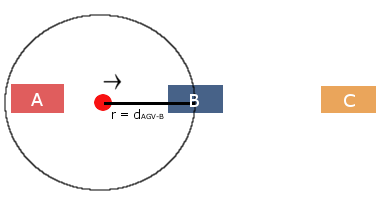
\includegraphics[width=10cm, height = 6cm]{negativeMotion.png}
  \caption{Cenário demonstrativo de um movimento no sentido negativo possível.}
  \label{negativeMotion}
\end{figure}

Pode-se observar na figura \ref{negativeMotion} o seguinte cenário: um AGV dirige-se a B para carregar um lote e levá-lo para C. Quando se encontra a meio do caminho, A requer um serviço de transporte até B. O AGV calcula a sua distância a B. A encontra-se dentro do círculo com raio igual a essa distância. Depois de fazer novos cálculos com a fórmula \ref{eqCusto}, o AGV decide ir a A antes de ir a B. Desta forma, o AGV faz o percurso A->B->C satisfazendo tanto o pedido de B como o de A, o que lhe faz poupar bateria e aumenta a eficiência do escoamento de pedidos.\newline

Qualquer pedido efetuado por máquinas fora do círculo não serão considerados pelo AGV por nunca valerem a pena nem em termos de bateria para o AGV nem em termos de eficiência da unidade de produção.

\subsection{Objectivos}
\justify\normalsize
O maior objectivo inerente a esta simulação é o de verificar a possibilidade de automação de uma unidade fabril por forma a diminuir a interação humana o mínimo possivel e visando obter a maior eficiência possivel na produção. Do ponto de vista da aplicação de agentes o ponto mais evidente é a observação da comunicação e do comportamento de e entre agentes máquina e AGV. Para além disto, um dos objectivos é a aplicação dos protocolos de negociação abordados na unidade curricular.

Será assumido na simulação que é do interesse da fábrica obter a maior eficiência possível na sua linha de produção. Isto significa que todas as escolhas de agentes terão em vista obter uma maior produtividade.

\subsection{Avaliação dos resultados} \label{ssec:evaluation}
\justify\normalsize
Os resultados serão avaliados através da construção de estatísticas das seguintes variáveis:

\begin{enumerate}
\item Tempo médio de processamento dos lotes\footnote{Um lote é considerado processado depois de ter passado por todas as fases de produção.};
\item Intervalo médio de negociação máquina-máquina;
\item Intervalo médio de negociação máquina-AGV;
\item Número de lotes processados dentro do tempo limite.
\end{enumerate}

Pretende-se comparar cenários com elevado número de máquinas e AGV's contra reduzido número dos mesmos. Pretende-se também testar cenários com variadas máquinas da mesma fase com capacidade e velocidade de processamento totalmente diferentes. Um cenário a explorar será um com opções de máquinas da mesma fase com elevada capacidade e reduzida velocidade e vice-versa.

Pretende-se ainda fazer uma análise comparativa entre cenários da quantidade de lotes processados num determinado intervalo de tempo estabelecido.

\subsection{Resultados esperados}
\justify\normalsize
Espera-se que o sistema tenha uma boa performance para situações baseadas no mundo real (unidades de produção médias e grandes). Antecipa-se que o intervalo de negociação máquina-AGV seja maior do que o tempo de negociação máquina-máquina devido à necessidade de cálculo de todos os caminhos possíveis.\newline 

Espera-se que em certos cenários a execução se torne mais lenta. Considera-se que os fatores que mais podem influenciar o tempo de execução são os seguintes:

\begin{enumerate}
\item Número elevado de máquinas e de AGV's no cenário;
\item Grande afluência de pedidos praticamente ou totalmente simultâneos.
\end{enumerate}


%----------------------------------------------------------------------------------------
%	JADE, REPAST+SaJas
%----------------------------------------------------------------------------------------

\section{Ferramentas}

\subsection{\textit{Overview} das plataformas a usar}
Para o desenvolvimento deste projecto serão utilizadas as ferramentas JADE, Repast Symphony e SAJaS. A linguagem de programação usada será JAVA.

\begin{description}
\item[JADE] Criação e definição de agentes.
\item[Repast Simphony] Simulação de agentes.
\item[SAJaS] Plataforma que possibilita a integração de agentes JADE com Repast.
\end{description}

O Repast Simphony é uma ferramenta importante na simulação de agentes pois permite simulações de MAS (\textit{Multi-agent Systems}) e visualização de gráficos com a informação colecionada durante as simulações. Esta plataforma tem uma interface gráfica intuitiva e extremamente interessante.

O SAJaS é também um componente chave pois permite integrar agentes JADE em simulações REPAST. Esta ferramenta permite juntar o melhor dos dois mundos: a construção de sistemas de agentes do JADE com o poder visual das simulações do REPAST. A maior vantagem de usar o SAJaS para integrar estas duas plataformas é o facto de permitir usar o poder do JADE de criação de agentes - o sistema das páginas amarelas, os comportamentos de agentes e a comunicação com protocolos FIPA - e poder simular vários agentes ao mesmo tempo com o REPAST, incluindo uma interface gráfica extremamente útil.

\subsubsection{Funcionalidades Relevantes}

O Repast Simphony tem uma componente visual muito forte (interface gráfica) o que facilita a visualização do comportamento de agentes num espaço físico, o que é extremamente interessante para projectar o espaço físico da unidade fabril e verificar o movimento dos AGV's. Para além disto, a plataforma será muito importante pois permitirá visualizar os indicadores chave da performance dos agentes especialmente as estatísticas referidas no ponto \ref{ssec:evaluation} que irão ser relevantes para a avaliação do sistema.

Os aspectos mais relevantes do JADE serão os \textit{behaviours} para definir os comportamentos, o \textit{Directory Facilitator} para tomar conhecimento de todos os agentes ativos e os seus AID's e os protocolos de comunicação FIPA para facilitar a comunicação e negociação entre agentes.


%----------------------------------------------------------------------------------------
%	Agentes
%----------------------------------------------------------------------------------------

\section{Sistema}

\subsection{Identificação e caracterização dos agentes}
O sistema será composto por dois tipos de agentes diferentes: \textbf{máquina} e \textbf{AGV}.

\begin{description}
\item[Máquina] - Agente representativo de uma máquina da linha de produção. Processa lotes, negoceia com máquinas da fase de produção seguinte e comunica com AGV's por forma a escolher o transporte do lote para a fase seguinte.
\item[AGV] - Agente representativo de um AGV. Comunica com máquinas, respondendo com os custos das deslocações. Se for requerido, transporta lotes entre máquinas.
\end{description}

Os comportamentos que os agentes podem ter estão especificados na tabela \ref{tableBehaviour}.

\begin{table}[H]
\centering
\caption{Comportamentos possíveis dos agentes.}
\label{tableBehaviour}
\begin{tabular}{@{}lll@{}}
\toprule
\multicolumn{1}{c}{\textbf{Comportamento}} & \textbf{Descrição} & \textbf{Agentes}      \\ \midrule
\multicolumn{1}{c}{Processar lotes}& Processo de processamento de um lote. & Máquina      \\ \midrule
\multicolumn{1}{c}{Negociar fase seguinte} & \begin{tabular}[c]{@{}l@{}}Negociação para escolher a máquina da fase seguinte \\ que vai processar o lote.\end{tabular} & Máquina      \\ \midrule
\multicolumn{1}{c}{Negociar transporte}    & Negociação do melhor AGV para efetuar o transporte.                           & Máquina, AGV \\ \midrule
\multicolumn{1}{c}{Movimento} & Qualquer movimentação feita no espaço físico.                                 & AGV          \\ \midrule
\multicolumn{1}{c}{Carregamento} & \begin{tabular}[c]{@{}l@{}}Passagem de carga da máquina que requer o transporte \\ para um AGV.\end{tabular} & Máquina, AGV \\ \midrule
\multicolumn{1}{c}{Entrega}  & Passagem da carga do AGV para a máquina destino.                              & Máquina, AGV \\ \midrule
\multicolumn{1}{c}{Recarregamento}  & Recarregamento da bateria na estação.                                         & AGV  \\ \bottomrule  
\end{tabular}
\end{table}

\subsection{Interação entre agentes}
A comunicação entre agentes será efetuada com o auxílio de mensagens JADE tomando proveito dos protocolos FIPA. Para cada agente tomar conhecimento de todos os outros agentes ativos e para obter os seus AID's será utilizado o \textit{Directory Facilitator} (DF) do JADE.\newline

\begin{lstlisting}
// Message sender API pseudo-code for FIPA INFORM type
public class Sender extends Agent {
	protected void send(String content, ArrayList AID_receivers){
		ACLMessage msg = new ACLMessage( ACLMessage.INFORM );
		msg.setContent(content);
		msg.addReceiver(AID_receiver); 
       // add more receivers if needed
		send(msg);
    }
}
\end{lstlisting}

\begin{lstlisting}
// Message receiver API pseudo-code for FIPA INFORM type
public class Receiver extends Agent {
	protected void setup() {
    	addBehaviour(new CyclicBehaviour(this) {
        	public void action() {
            	ACLMessage msg= receive();
                if (msg!=null)
                	reply(msg);
                else
					<... do something else ...>
             }
		});
	}
    protected void reply(ACLMessage msg){
    	ACLMessage reply = msg.createReply();
        reply.setPerformative( ACLMessage.INFORM );
        reply.setContent("Message content" );
        reply.send();
    }
}
\end{lstlisting}

Ao ser iniciada uma simulação, todos os agentes máquina fazem \textit{broadcast} da sua localização e a fase de produção a que pertencem. Cada agente guarda desta interação inicial a informação importante às suas tarefas. Agentes máquina guardam os AIDs de todas as máquinas da fase seguinte à sua. Os AGV's guardam a localização de todas as máquinas.\newline

As interações entre agentes podem ser de dois tipos:

\begin{enumerate}
\item Máquina - máquina;
\item Máquina - AGV.
\end{enumerate}

\subsubsection{Protocolo máquina-máquina}

\textbf{FALTA ISTO!!!!!!!!!!!!!!!}

\subsubsection{Protocolo máquina-AGV}

\textbf{FALTA ISTO!!!!!!!!!!!!!!!!!}

\subsection{Faseamento}
Prevê-se que o projeto seja desenvolvido segundo as fases especificadas em baixo.

\begin{enumerate}
\item Desenvolvimento dos agentes máquina;
\item Implementação do protocolo de negociação máquina-máquina;
\item Desenvolvimento dos agentes AGV;
\item Implementação do protocolo de negociação máquina-AGV;
\item Simulação de variados cenários;
\item Avaliação e comparação estatística dos resultados.
\end{enumerate}

\section{Conclusões}
\justify\normalsize
Conclui-se que o sistema planeado é extremamente relevante, tendo um papel importante no aprofundamento do conhecimento de agentes de inteligência artificial. Na realidade, a utilização das ferramentas referidas no documento ajuda a compreender os âmbitos de agentes, os processos de construção e simulação dos mesmos. A inteligência artificial é cada vez mais um factor de extrema importância à vida humana, em facto, tem-se espalhado por todos os cantos do mundo, tomando de assombro todos os dispositivos tecnológicos. Esta disciplina já é mais do que um sonho, é algo concreto, possível, algo que desafia aquilo que se achavam serem as leis da vida e da inteligência. O facto de que este projecto possa ter um âmbito do mundo real é um factor de motivação e apela ao seu desenvolvimento.

\bibliography{title_page_1}
\bibliographystyle{plain}

\end{titlepage}
\end{document}